\documentclass[11pt,aspectratio=43]{beamer}
\usepackage{tikz}
\usetheme{Madrid}
\setbeamertemplate{navigation symbols}{}
\title{Geometric uncertainty: experiments and bounds}
\subtitle{Generated interaction study}
\author{Research group}
\date{}
\year=2026\month=11\day=5
\newcommand{\fuzzlayerA}[1]{\textrm{#1}}
\newcommand{\fuzzlayerB}[1]{\fuzzlayerA{#1}}
\newcommand{\fuzzterm}[1]{\fuzzlayerB{#1}}
\newcommand{\fuzzpair}[2]{\fuzzterm{#1}: #2}
\newcommand{\fuzzunit}{ms}
\let\fuzzoriginalunit\fuzzunit
\newcommand{\fuzzcoefficient}{1}
\newcommand{\fuzzscale}[2][\fuzzcoefficient]{#1\,#2}
\definecolor{fuzzpaint}{RGB}{255,0,255}
\definecolor{fuzzsecond}{RGB}{18,137,67}
\tikzset{fuzzvertex/.style={draw,rounded corners=1pt,fill=blue!10,inner sep=1pt,minimum width=.35cm,minimum height=.25cm}}
\begin{document}
\section{Geometric uncertainty}
\begin{frame}[t,shrink=5]{Geometric uncertainty}{Composed dependencies}
\fuzzpair{Experiment}{Timing: 12\fuzzunit; estimate $\fuzzscale{x}+\fuzzscale[2]{y}$.}\par
{\renewcommand{\fuzzunit}{samples}\let\fuzzterm\textit\fuzzpair{LocalScope}{Timing: 7\fuzzunit.}\par}
\fuzzpair{RestoredScope}{Timing: 11\fuzzunit.}\par
\begin{itemize}
\item<1-> \begin{enumerate}
\item<1-> \visible<2-3>{\[\begin{aligned}a+b&=c\\ d-e&=f\end{aligned}\]}
\item<2-> \begin{description}
\item[Stage 1] \textrm{We compare the} proposed solution with a reference computed from the complete input.  The estimate is $\sum_{i=1}^{n}x_i$.
\item[Stage 2] 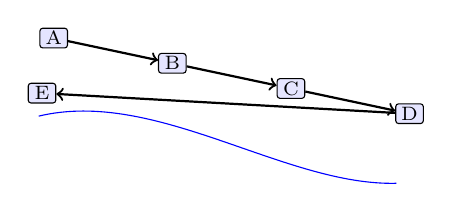
\begin{tikzpicture}[font=\scriptsize]
\begin{scope}[scale=1.1,rotate=-12]


\node[fuzzvertex] (g6n0) at (0.000,0) {A};
\node[fuzzvertex] (g6n1) at (1.400,0) {B};
\node[fuzzvertex] (g6n2) at (2.800,0) {C};
\node[fuzzvertex] (g6n3) at (4.200,0) {D};
\node[fuzzvertex] (g6n4) at (0.000,-0.65) {E};
\begin{scope}[xshift=.5pt,yshift=-.5pt]
\draw<1->[->,thick] (g6n0) -- (g6n1);
\draw<1->[->,thick] (g6n1) -- (g6n2);
\draw<1->[->,thick] (g6n2) -- (g6n3);
\draw<1->[->,thick] (g6n3) -- (g6n4);
\draw[blue] (0,-.9) .. controls (1.260,-.3) and (2.940,-1.1) .. (4.200,-.8);
\end{scope}
\end{scope}
\end{tikzpicture}
\end{description}
\item<3-> {\footnotesize\color{black}\raggedleft
\textit{A local update} can change the measurements used by several neighboring components. A narrow column can change line breaking even when the underlying expression is unchanged. The estimate is $\alpha+\beta$.\par}
\end{enumerate}
\item<2-> \begin{itemize}
\item<1-> \alt<1-2>{\begin{itemize}
\item<1-> \textit{The final diagram} records the order in which information crosses the partition. A narrow column can change line breaking even when the underlying expression is unchanged. The estimate is $\alpha+\beta$.
\item<2-> \begin{tabular}{lrr}Method&Cost&Error\\\hline
Fresh0&10&2\\
Global1&10&6\\
\end{tabular}
\end{itemize}}{Alternative estimate $x_0$.}
\item<2-> \begin{columns}[onlytextwidth,T]
\begin{column}{0.54\textwidth}
\[\begin{aligned}a+b&=c\\ d-e&=f\end{aligned}\]
\end{column}
\begin{column}{0.42\textwidth}
\textrm{We compare the} proposed solution with a reference computed from the complete input. A narrow column can change line breaking even when the underlying expression is unchanged. The estimate is $\sum_{i=1}^{n}x_i$.
\end{column}
\end{columns}
\end{itemize}
\item<3-> \begin{columns}[onlytextwidth,b]
\begin{column}{0.46\textwidth}
\begin{alertblock}{Cache invalidation}
\begin{enumerate}
\item \[\begin{pmatrix}a&b\\c&d\end{pmatrix}\begin{pmatrix}x\\y\end{pmatrix}\]
\item \begin{tabular}{lrr}Method&Cost&Error\\\hline
Cached0&9&17\\
Local1&10&13\\
\end{tabular}
\end{enumerate}
\end{alertblock}
\end{column}
\begin{column}{0.50\textwidth}
\begin{columns}[onlytextwidth,b]
\begin{column}{0.54\textwidth}
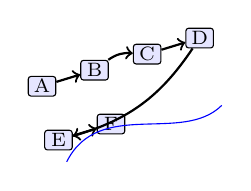
\begin{tikzpicture}[font=\scriptsize]
\begin{scope}[scale=1.1,rotate=17]


\node[fuzzvertex] (g23n0) at (0.000,0) {A};
\node[fuzzvertex] (g23n1) at (0.634,0) {B};
\node[fuzzvertex] (g23n2) at (1.269,0) {C};
\node[fuzzvertex] (g23n3) at (1.903,0) {D};
\node[fuzzvertex] (g23n4) at (0.000,-0.65) {E};
\node[fuzzvertex] (g23n5) at (0.634,-0.65) {F};
\begin{scope}[xshift=.5pt,yshift=-.5pt]
\draw<1->[->,thick] (g23n0) -- (g23n1);
\draw<1->[->,thick] (g23n1) to[bend left=20] (g23n2);
\draw<1->[->,thick] (g23n2) -- (g23n3);
\draw<1->[->,thick] (g23n3) to[bend left=20] (g23n4);
\draw<1->[->,thick] (g23n4) -- (g23n5);
\draw[blue] (0,-.9) .. controls (0.571,-.3) and (1.332,-1.1) .. (1.903,-.8);
\end{scope}
\end{scope}
\end{tikzpicture}
\end{column}
\begin{column}{0.42\textwidth}
\textbf{A narrow column} can change line breaking even when the underlying expression is unchanged.  The estimate is $\frac{a+b}{1+c}$.
\end{column}
\end{columns}
\end{column}
\end{columns}
\end{itemize}
\par 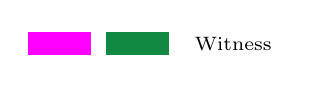
\begin{tikzpicture}[font=\scriptsize]
\fill<2-3>[fuzzpaint] (0,0) rectangle (.8,.3);
\fill<3->[fuzzsecond] (1,0) rectangle (1.8,.3);
\node[anchor=west] at (2,0.15) {Witness};
\end{tikzpicture}
\only<5>{}
\end{frame}
\renewcommand{\fuzzunit}{min}
\renewcommand{\fuzzcoefficient}{2}
\renewcommand{\fuzzterm}[1]{{\textrm{#1}}}
\section{Constraint propagation}
\begin{frame}[t]{Cache invalidation}
\fuzzpair{MacroStageB}{Timing: 12\fuzzunit, retained: 9\fuzzoriginalunit.}\par
{\renewcommand{\fuzzunit}{local}\fuzzpair{FrameLocal}{Timing: 5\fuzzunit.}\par}
\fuzzpair{FrameRestored}{Timing: 8\fuzzunit; estimate $\fuzzscale{x}$.}\par
\begin{columns}[T]\begin{column}{.46\textwidth}A narrow column can change line breaking even when the underlying expression is unchanged.\end{column}\begin{column}{.46\textwidth}\begin{itemize}\item Input state\item Updated state\end{itemize}\end{column}\end{columns}
\end{frame}
\renewcommand{\fuzzunit}{s}
\renewcommand{\fuzzcoefficient}{3}
\renewcommand{\fuzzterm}[1]{{\textbf{#1}}}
\section{Incremental analysis}
\begin{frame}[t]{Iterative refinement}
\fuzzpair{MacroStageC}{Timing: 12\fuzzunit, retained: 9\fuzzoriginalunit.}\par
{\renewcommand{\fuzzunit}{local}\fuzzpair{FrameLocal}{Timing: 5\fuzzunit.}\par}
\fuzzpair{FrameRestored}{Timing: 8\fuzzunit; estimate $\fuzzscale{x}$.}\par
\begin{block}{Follow-up}\fuzzterm{A revised value} depends on the preceding frame.\end{block}
\[r_{k+1}=r_k-\alpha d_k\]
\end{frame}
\renewcommand{\fuzzunit}{min}
\renewcommand{\fuzzcoefficient}{4}
\renewcommand{\fuzzterm}[1]{{\textrm{#1}}}
\section{Message passing}
\begin{frame}[t]{Geometric uncertainty}
\fuzzpair{MacroStageD}{Timing: 12\fuzzunit, retained: 9\fuzzoriginalunit.}\par
{\renewcommand{\fuzzunit}{local}\fuzzpair{FrameLocal}{Timing: 5\fuzzunit.}\par}
\fuzzpair{FrameRestored}{Timing: 8\fuzzunit; estimate $\fuzzscale{x}$.}\par
\begin{columns}[T]\begin{column}{.46\textwidth}The next pass must preserve the boundary conditions while revisiting dependent values.\end{column}\begin{column}{.46\textwidth}\begin{itemize}\item Input state\item Updated state\end{itemize}\end{column}\end{columns}
\end{frame}
\end{document}
